
%(BEGIN_QUESTION)
% Copyright 2015, Tony R. Kuphaldt, released under the Creative Commons Attribution License (v 1.0)
% This means you may do almost anything with this work of mine, so long as you give me proper credit

En svært vanlig transformator i industrielle styrekretser er \textit{control power transformer}, vist både som bilde og skjemategning.  Primærviklingen består oftest av \textit{to} spoler som kan kobles ulikt avhengig av tilgjengelig AC-forsyningsspenning:

$$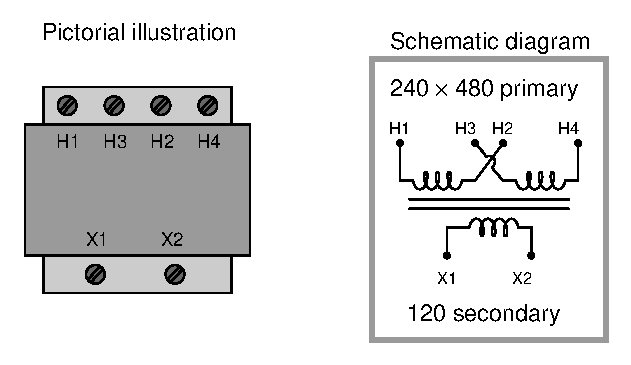
\includegraphics[width=15.5cm]{i00267x01.eps}$$

Bestem først hvordan 240 VAC kobles til primærterminalene.  Bestem deretter hvordan høyere linjespenning på 480 VAC kobles til primærterminalene.

\vskip 10pt

Forklar så hvordan et multimeter kan brukes til å teste viklingene, både for \textit{åpne} og \textit{kortsluttede} feil.

\vskip 10pt

Til slutt: forklar hvordan testutstyret \textit{isolasjonstester} (ofte kalt ``Megger'') brukes til å sjekke viklingene for jordfeil (til transformatorens jernkjerne), og hvordan dette testutstyret skiller seg fra et vanlig ohmmeter.


\vskip 20pt \vbox{\hrule \hbox{\strut \vrule{} {\bf Forslag til sokratisk diskusjon} \vrule} \hrule}

\begin{itemize}
\item{} Forklar hvorfor H2/H3-terminalene er ``krysset'' slik de vises i skjemaet.
\item{} Bestem hvordan transformatoren kunne blitt redesignet for både to sekundærspenningsvalg (240 VAC vs. 120 VAC) og to primærspenningsvalg.
\end{itemize}

\underbar{file i00267}
%(END_QUESTION)





%(BEGIN_ANSWER)

$$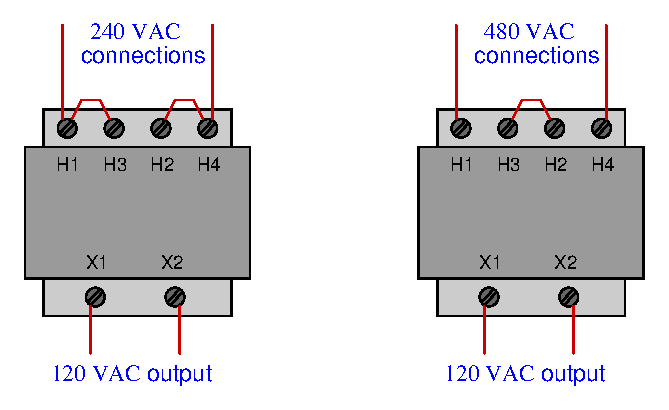
\includegraphics[width=15.5cm]{i00267x02.eps}$$

Jeg lar deg selv bestemme hvordan et multimeter brukes for viklingstester i en styrestrømtransformator.

\vskip 10pt

En \textit{megger} er et spesielt høyohmig ohmmeter som bruker testspenning på flere hundre eller tusen volt.  Den kan oppdage feil i viklingsisolasjon i multi-megaohm-området.

%(END_ANSWER)






%(BEGIN_NOTES)

For å oppdage en \textit{åpen} feil må du måle høy motstand mellom punkter som egentlig skal være sammenkoblet (f.eks. H1-H2, H3-H4, X1-X2).

\vskip 10pt

For å oppdage en \textit{kortsluttet} feil må du måle unormalt lav motstand mellom punkter (f.eks. H1-H2, H3-H4, X1-X2, mellom en terminal og jernkjerne).

%INDEX% Electronics review: megger (test equipment)
%INDEX% Troubleshooting review: electric circuits

%(END_NOTES)
